\documentclass[11pt,twoside]{article}

\usepackage[paperheight=9in,paperwidth=6in]{geometry}
%\pagenumbering{gobble}
\usepackage{fontspec}
\usepackage{fancyhdr}
\usepackage{needspace}
\usepackage{graphicx}
\usepackage[autocompile]{gregoriotex}
\def\GreStar{*}
%\gresetheadercapture{annotation}{greannotation}{string}

\setmainfont{EB Garamond}[UprightFont=EB Garamond Regular,
ItalicFont= EB Garamond Italic,
BoldFont= EB Garamond Bold,
Ligatures=Rare,
StylisticSet=6,
Numbers=Proportional,
Numbers=OldStyle]
\newfontfamily{\medium}{EB Garamond Medium}

\pagestyle{fancy}
\fancyhead{}
\fancyfoot{}
\renewcommand{\headrulewidth}{0pt}

\fancyhead[RO]{\small\rightmark\hspace{1cm}\thepage}
\fancyhead[LE]{\small\thepage\hspace{1cm}\leftmark}

\newcommand{\setheaders}[2]{
	\renewcommand{\rightmark}{{\sc#2}}
	\renewcommand{\leftmark}{{\sc#1}}
}
\setheaders{}{}

\newcommand{\officiumtitulum}[1]{
  \newpage
  \thispagestyle{empty}
  \setheaders{{\addfontfeature{LetterSpace=5.0} #1}}{{\addfontfeature{LetterSpace=5.0} #1}}
  \begin{center}
  {\LARGE\addfontfeature{LetterSpace=5.0} #1}\par
  \end{center}
}

\newcommand{\smalltitle}[1]{
\needspace{5\baselineskip}
\vspace{\baselineskip}
 {\centering #1\par}
}

\begin{document}

%\begin{titlepage}
% \begin{center}
% \fontsize{36}{45}\selectfont{D\textsc{ominica}\\ A\textsc{d} V\textsc{esperas}}
% \end{center}
%\centering
%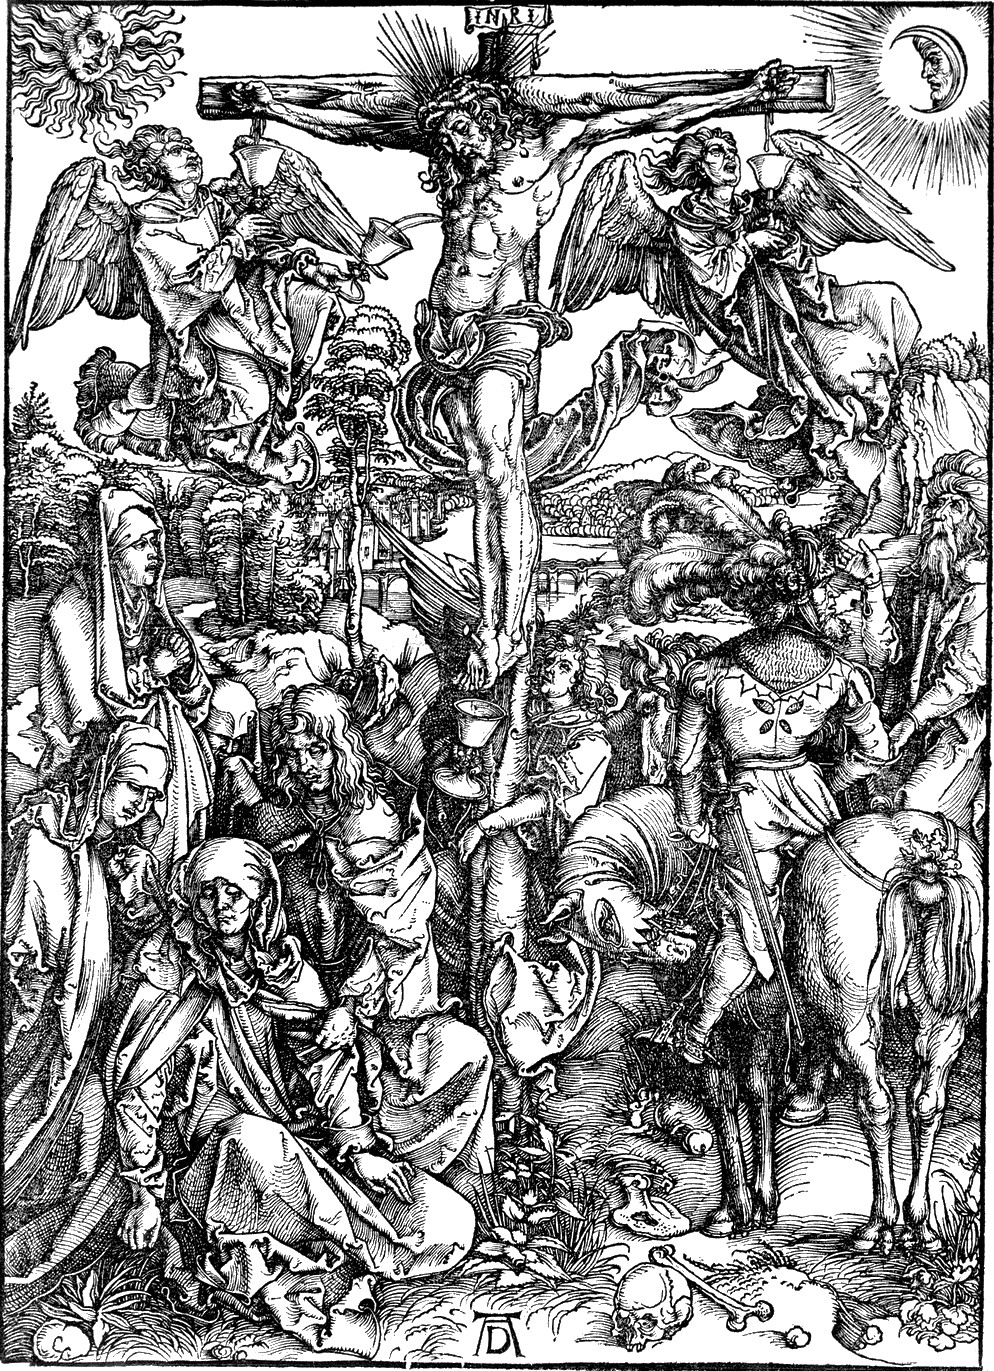
\includegraphics[width=10cm,height=10cm,keepaspectratio]{Durer,_la_grande_passione_06}
% \begin{center}
% \fontsize{36}{45}\selectfont{T\textsc{empore} P\textsc{assionis}}
% \end{center}
%\end{titlepage}
%\newpage\null\thispagestyle{empty}\newpage

%\begin{center}Dominica Passionis\end{center}
\officiumtitulum{DOMINICA PASSIONIS}
\begin{center}Capitulum\end{center}

\begin{flushright}{\fontsize{9}{11}\selectfont{Heb. 9:11-12}}\end{flushright}
Fratres: Christus assístens Póntifex futurórum bonórum, per ámplius et perféctius tabernáculum non manu factum, id est, non huius creatiónis:~† neque per sánguinem hircórum aut vitulórum, sed per próprium sánguinem introívit semel in Sancta, * ætérna redemptióne invénta.

℟. Deo grátias.

\smalltitle{Hymnus}
%\greannotation{1.}
\grechangestyle{initial}{\fontsize{28}{28}\selectfont}
\gregorioscore{Vexilla_regis_prodeunt}
\bigskip

\gresetinitiallines{0}
\gregorioscore{Versus_Temporis_Passionis}
\noindent \hspace*{-0,2mm} ℟ . \hspace{14.3mm}A \hspace{3.2mm}víro \hspace{3.2mm}iníquo \hspace{3.2mm}éripé \hspace{5.9mm}me.
\bigskip

\gresetinitiallines{1}
\grechangedim{annotationseparation}{-0.01cm}{fixed}
%\greannotation{Ad Magnif.}
%\greannotation{Ant. 2. D}
\grechangestyle{initial}{\fontsize{28}{28}\selectfont}
\gregorioscore{Abraham_pater_vester}

\smalltitle{Oratio}
Orémus.\\ 
Quǽsumus, omnípotens Deus, famíliam tuam propítius réspice: † ut, te largiénte, regátur in córpore; * et, te servánte, custodiátur in mente. Per Dóminum nostrum Jesum Christum, Fílium tuum: qui tecum vivit et regnat in unitáte Spíritus Sancti, Deus, per ómnia sǽcula sæculórum.

℟. Amen.

\newpage
%\begin{center}Dominica in Palmis\end{center}
\officiumtitulum{DOMINICA IN PALMIS}
\begin{center}Capitulum\end{center}

\begin{flushright}{\fontsize{9}{11}\selectfont{Phil. 2:5-7}}\end{flushright}
Fratres: Hoc enim sentíte in vobis, quod et in Christo Jesu: qui, cum in forma Dei esset, non rapínam arbitrátus est esse se æquálem Deo: † sed semetípsum exinanívit, formam servi accípiens, in similitúdinem hóminum factus, * et hábitu invéntus ut homo.

℟. Deo grátias.
\bigskip
%\greannotation{Ad Magnif.}
%\greannotation{Ant. 8. G}
\grechangestyle{initial}{\fontsize{28}{28}\selectfont}
\gregorioscore{Scriptum_est_enim__percutiam}

\newpage

\smalltitle{Oratio}
Orémus.\\ 
Omnípotens sempitérne Deus, qui humáno géneri, ad imitándum humilitátis exémplum, Salvatórem nostrum carnem súmere, et crucem subíre fecísti: † concéde propítius; ut et patiéntiæ ipsíus habére documénta,*  et resurrectiónis consórtia mereámur.
Per eúndem Dóminum nostrum.

℟. Amen.

\enddocument